% overleaf document: measured noise spectrum2 simulations with some small modifications. Also use passive voice instead of "we". 
%% plots are produced: cernbox/Project_thesis/scripts_for_simple_figures_plots (also at /eos/user/n/natriant/2018/CC_MD_2018_summary/measured_psd/job000). and for Fig.6 /eos/user/n/natriant/pyheadtail_data/9July2021. 

This appenidx discusses the basic terminology of signal processing and gives the definitions which are used in this thesis. The focus is on Fourier transform and the power spectral density. First the most general mathematical definitions which concern signals continuous in time and with infinite time duration are discussed. Secondly, the definitions are given for signals sampled at a finite number of points, which are considered for the measurements and for the computational analysis. Furthermore, the quantities that are used most often for noise power spectrum measurements and their relationship to the mathematical definitions of the power spectral density are discussed. Finally, the way of applying a measured noise spectrum in numerical simulations is described.

\section{Continuous-time analysis}\label{app:continuous_time_analysis}
\subsubsection*{Fourier transform} %\hfill \break
A physical process (or signal or time series) can be described in the time domain by a continuous function of time, e.g.~$y(t)$, or else in the frequency domain, where the process is specified by giving its amplitude $\fourierxform{y}$ as a function of frequency, e.g.~$\fourierxform{y}(f)$ with $f \in \left(-\infty, +\infty \right )$. In other words, $y(t)$ and $\fourierxform{y}(f)$ are essentially different representations of the same function.  In general, $\fourierxform{y}(f)$ can be a complex quantity, with the complex argument giving the phase of the component at the frequency $f$.

One can switch between these two representations using the Fourier transform method. In this thesis the Fourier transform of a time series $y(t)$, which will be denoted in this document by $\fourierxform{y}$, is defined as~\cite{a_numerical_recipies}: %eq.12.0.1

\begin{equation}\label{eq:fft_definition}
\fourierxform{y}(f) = \int_{-\infty}^{\infty} y(t) e^{-2\pi \imagunit t f} dt,
\end{equation}
where $f$ stands for any real number. 
If the time is measured in seconds the frequency, $f$, is measured in Hertz. 

The inverse Fourier transform, which is used to re-create the signal from its spectrum, is defined as~\cite{a_numerical_recipies}:
\begin{equation}\label{eq:ifft_definition}
y(t) = \int_{-\infty}^{\infty} \fourierxform{y}(f) e^{2\pi \imagunit t f} df.
\end{equation}

\subsubsection*{Power spectral density and total power} %\hfill \break
The power spectral density (PSD), $S_{yy}(f)$, of a signal (or a time series), $y(t)$ it describes the distribution of the power in a signal between its frequency components, and is defined as the Fourier transform of the autocorrelation function, $R_{yy}(t)$~\cite{b_papoulis1991probability}: % Eq.10-14 p. 338
%"Autocorrelation" is used to compare a signal with a time-delayed version of itself. If a signal is periodic, then the signal will be perfectly correlated with a version of itself if the time-delay is an integer number of periods.

\begin{equation}\label{eq:Sxx_definition}
    S_{yy}(f) = \fourierxform{R}_{yy}(f) =  \int_{-\infty}^{\infty} R_{yy}(\tau)e^{-2\pi \imagunit \tau f} d\tau.
\end{equation}

The continuous autocorrelation $R_{yy}(\tau)$ is defined as the continuous cross-correlation integral of $y(t)$ with itself, at lag $\tau$~\cite{FFT_and_applications}:
\begin{equation}\label{eq:Rxx_definition}
    R_{yy}(\tau) = (y \ast y)(\tau) = \int_{-\infty}^{\infty} \bar{y}(t) y(t+\tau) dt,
\end{equation}
where $\ast$ denotes the convolution operation and $\bar{y}(t)$ represents the complex conjugate of $y(t)$.

% cross (lagged) correlation
According to the cross-correlation theorem \cite{FFT_and_applications}:
\begin{equation}\label{eq:cross_correlation_theorem}
\fourierxform{R}_{yy}(f) = \bar{\fourierxform{y}}(f) \fourierxform{y}(f) = \mid \fourierxform{y}(f) \mid ^2,
\end{equation}
where $\fourierxform{y}(f)$ is the Fourier transform of the signal as defined in Eq.~(\ref{eq:fft_definition}).

From Eq.~(\ref{eq:Sxx_definition}) and Eq.~(\ref{eq:cross_correlation_theorem}) the power spectral density of a signal $y(t)$ can be simply written as the square of its Fourier transform:
\begin{equation}\label{eq:Sxx_definition_v2}
S_{yy}(f) = \mid \fourierxform{y}(f) \mid ^2,
\end{equation}
with  $f \in \left(-\infty, +\infty \right )$.

\section{Discrete-time analysis}\label{app:discrete_time_analysis}

\subsubsection*{Discrete-time signals} %\hfill \break
% the following paragraph is from here: https://sceweb.sce.uhcl.edu/harman/ceng5431/2015WEB/Chap11tlhDFT.pdf
Figure~\ref{fig:sampling_of_continuous_signal} shows a part of a continuous signal $y(t)$. For signal measurements and computational analysis, signals (or time series) sampled at a finite number of points are considered. Such signals are called discrete-time signals and typically they are sampled at equal points in time. For example, in Figure~\ref{fig:sampling_of_continuous_signal}, it is assumed that the continuous signal, $y(t)$, is sampled at intervals $\Delta t$ creating a set of $N$ points. The length in time between the first and final sample is $T_\mathrm{total} = N\Delta t$.

%$T_\mathrm{sample}=\frac{N-1}{N}T$, where $T = N\Delta t$. %One can see that the continuous signal is not only sampled but also truncated.

\begin{figure}[!ht]
     \centering         
     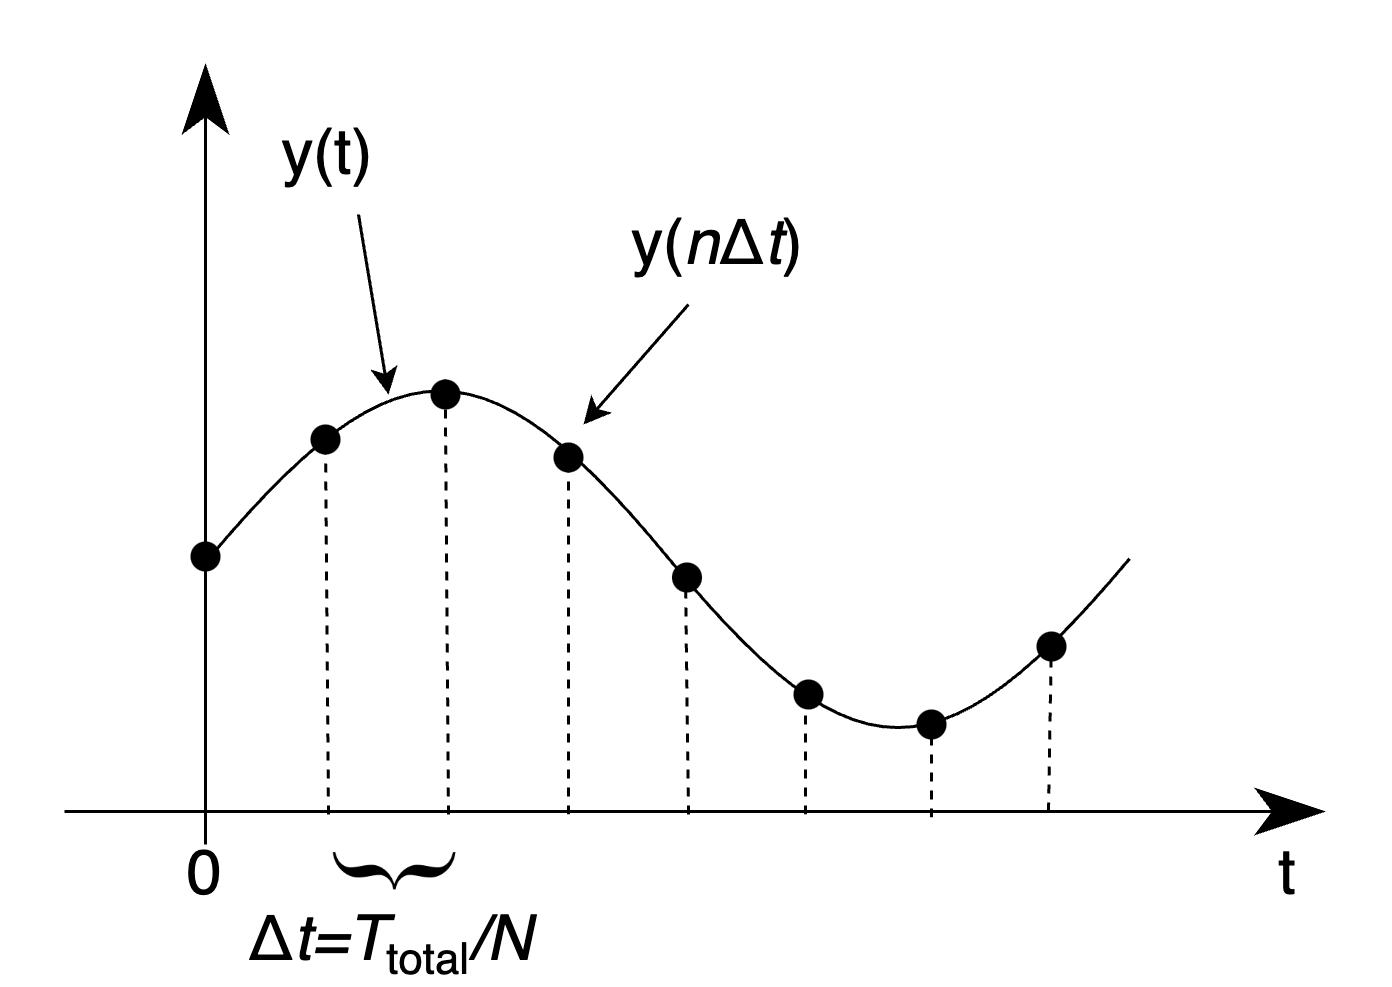
\includegraphics[width=0.6\textwidth]{./images/app_B/approximation_of_continuous_to_discrete_signal.png}
         \caption{Sampling of the continuous signal $y(t)$ at a finite number of points $N$. The sampled signal is the discrete-time signal $y(n\Delta t)$ with $\Delta t$ the sampling interval and  $n$ an integer such that $n \in \left[0,N-1 \right ]$.}
         \label{fig:sampling_of_continuous_signal}
\end{figure}

\subsubsection*{Discrete Fourier transform} %\hfill \break %\label{subsec:DFT}
Let us consider a discrete-time signal, $y_n$, which is sampled at $N$ consecutive samples, $y_n = y(n \Delta t)$, with $n \in \left[0,N-1 \right ]$ such that $\Delta t$ is the sampling interval. The following discussion considers that $N$ is an odd integer. The Fourier transform for a discrete time signal, also known as discrete Fourier transform, is given by~\cite{a_numerical_recipies}:%Chapter 12, Eq.(12.1.7)
% Link to reference: https://faculty.washington.edu/seattle/brain-physics/FFT/numerical-recipes.pdf
% Also check the abover eference for aliasing p.500 and 501
\begin{equation}\label{eq:DFT_definiton}
    \fourierxform{y}_k= \sum_{n=0}^{N-1} y(n\Delta t) e^{-2\pi \imagunit \frac{k n}{N}},
\end{equation}
where the index $k$ is an integer in the range $-\frac{N-1}{2}$ to $\frac{N-1}{2}$.


%As a first step, we note that the integral of Eq.~(\ref{eq:fft_definition}) can be represented by a discrete sum in the limit that $\Delta t \to 0$:
%\begin{equation}\label{eq:dft_proof}
%\fourierxform{y}(f) = \int_{-\infty}^{\infty} y(t) e^{-2\pi \imagunit f t} dt =
%\lim_{\Delta t \to 0}
%\sum_{n=-\infty}^\infty y(n\Delta t) e^{-2\pi \imagunit f n \Delta t} \Delta t.
%= \Delta t \sum_{n=0}^{N-1} y(n\Delta t) e^{\frac{-j 2\pi k n}{N}},
%\end{equation}
%where $f_k=k/(N\Delta t)$ and $k \in \left[-\frac{N-1}{2},+\frac{N-1}{2} \right ]$ (for odd $N$) or  $k \in \left[-\frac{N}{2},+\frac{N}{2} \right ]$ (for even $N$), and $k$ being an integer.

%Based on the expression for the summation in Eq.~(\ref{eq:dft_proof}), we define the discrete Fourier transform as follows~\cite{a_numerical_recipies}: % Chapter 12, Eq.(12.10)
%\begin{equation}\label{eq:DFT_definiton}
%\fourierxform{y}_k= \sum_{n=0}^{N-1} y(n\Delta t) e^{-2\pi \imagunit \frac{k n}{N}}.
%\end{equation}
%Here, the index $k$ is an integer in the range $-\frac{N-1}{2}$ to $\frac{N-1}{2}$.
%Each component $\fourierxform{y}_k$ of the discrete Fourier transform is related to the component $\fourierxform{y}(f)$ of the continuous Fourier transform of $y(t)$, for $f = k/T$, in the limit $\Delta t \to 0$ and $N \to \infty$ (and where it is assumed that $y(t) = 0$ for $t < 0$ and for $t > T$).

%It should be noted that the discrete Fourier transform is calculated only at integer values of $k$, and therefore for $N$ samples the discrete Fourier transform will consist of $N$ numbers. 

The components of the discrete Fourier transform are calculated at frequencies $f_k$ that are integer multiples of $\Delta f = 1/T_\mathrm{total} = f_s/N$, with $f_s = 1/\Delta t$ the sampling frequency. In that case, $f_k \in \left[-\frac{N-1}{2T_\mathrm{total}},\frac{N-1}{2T_\mathrm{total}} \right]$. An example of a discrete Fourier transform is shown in Fig.~\ref{fig:signal_and_DFT_example}.
%/Delta_f is the resolution frequency
\begin{figure}[!ht]
    \centering
    \begin{subfigure}[t]{0.45\textwidth}
        \centering
        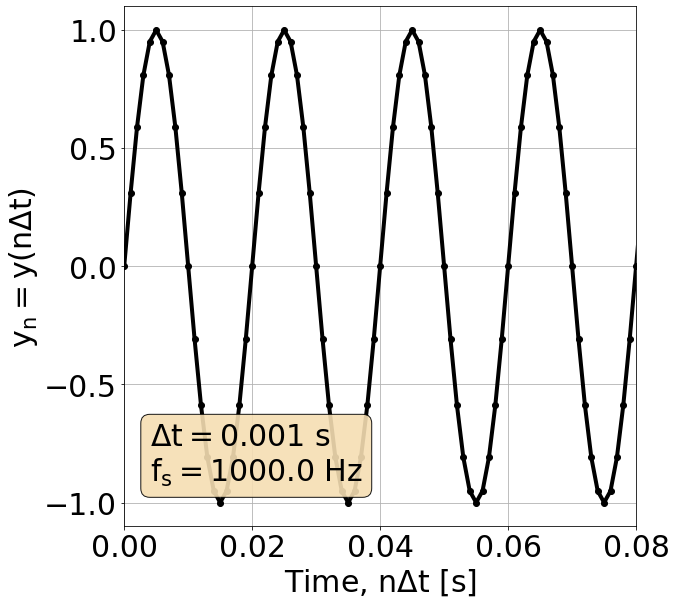
\includegraphics[width=1\textwidth]{./images/app_B/simple_signal_1freq_example.png}
        \caption{$y=\sin(2 \pi f t),\ f=50$ Hz}
        \label{fig:signal_and_DFT_example_a}
    \end{subfigure}
    \hfill
    \begin{subfigure}[t]{0.45\textwidth}
        \centering
        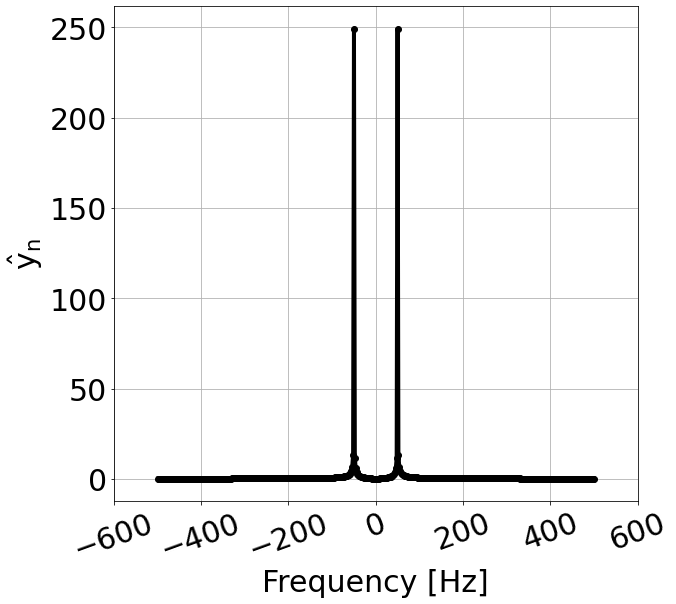
\includegraphics[width=1\textwidth]{./images/app_B/simple_signal_1freq_fft_example.png}
        \caption{Discrete Fourier transform}
        \label{fig:signal_and_DFT_example_b}
    \end{subfigure}
    \hfill
     \caption{Example of a signal sampled at discrete time intervals, and the corresponding discrete Fourier transform.}
     \label{fig:signal_and_DFT_example}
\end{figure}

When using this convension the Fourier tranfrom components outisde of the above mentioned frequency range are considered zero. Note that the zero frequency, $f_k=0$, corresponds to $n=0$. The positive frequencies, $0  < f_k < + \frac{N-1}{2T_\mathrm{total}}$ correspond to values $1 < n < (N-1)/2$ and the negative frequencies,  $-\frac{N-1}{2T_\mathrm{total}}  < f_k < 0$ correspond to values $(N-1)/2 < f_k < 0$. The value n = $(N-1)/2$ corresponds to both $f_k = - \frac{N-1}{2T_\mathrm{total}}$ and + $\frac{N-1}{2T_\mathrm{total}}$

% p.503 in the following link: https://faculty.washington.edu/seattle/brain-physics/FFT/numerical-recipes.pdf

The inverse discrete Fourier transform is defined as:
\begin{equation}\label{eq:iDFT_definiton}
 y_n =  y(n\Delta t) = \frac{1}{N} \sum_{k=-\frac{N-1}{2}}^{\frac{N-1}{2}} \fourierxform{y}_k e^{2\pi \imagunit \frac{k n}{N}},
\end{equation}
where $n \in \left[0,N-1 \right ]$ and where $n$ and $k$ are both integers.

The definitions given in Eq.~(\ref{eq:DFT_definiton}) and Eq.~(\ref{eq:iDFT_definiton}) are consistent with those used in numpy, in the numpy.fft function \cite{numpy_fft} package of the Python programming language. 

\subsubsection*{Power spectral density} % \hfill \break
Following Eq.~(\ref{eq:Sxx_definition_v2}) the power spectral density of a discrete-time signal should be estimated as follows:

\begin{equation}\label{eq:Sxx_definition_discrete_not_normalised}
    S_{yy}(f_k) = C_\mathrm{PSD} \mid \fourierxform{y}_k(f_k) \mid ^2,
\end{equation}
where $f_k \in \left[-\frac{N-1}{2T_\mathrm{total}},\frac{N-1}{2T_\mathrm{total}} \right]$. $C_\mathrm{PSD}$ is a normalisation constant which is introduced in order to obtain the correct amplitudes at each frequency and thus the correct noise power. There are several different conventions for the choice of this normalization. In this thesis, the following normalization is considered (more details in the following paragraph):
% I choose this normalisation as it gave the correct results in terms of noise power.
\begin{equation}\label{eq:Sxx_definition_discrete_normalized}
    S_{yy}(f_k) = \frac{1}{N^2 \Delta f} \mid \fourierxform{y}_k(f_k) \mid ^2,
\end{equation}
where  $\Delta f = 1/T_\mathrm{total}$ the frequency resolution and $N$ the number of samples.
    
\begin{figure}[!ht]
    \centering         
    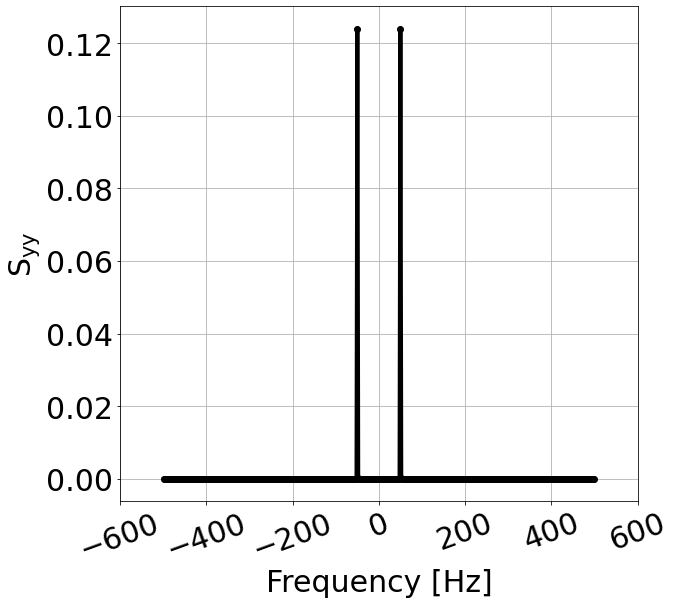
\includegraphics[width=0.5\textwidth]{./images/app_B/simple_signal_1freq_psd_example.png}
        \caption{Power spectrum of $y=\sin(2 \pi f t),\ f = $50\,Hz.}
        \label{fig:psd_example_two_sided}
\end{figure}

Figure~\ref{fig:psd_example_two_sided} shows an example power spectrum of the time-domain signal shown in Fig.~\ref{fig:signal_and_DFT_example}a. It can be seen that the spectrum that results from the analysis above is two-sided, which means that it has both positive and negative frequencies. It is also symmetric around the DC component ($f = $0\,Hz), which is a property of a real signal. 

The power spectral density is expressed in terms of the square of the amplitude of the signal per unit frequency. For example, for a signal defined in units of voltage, V, (e.g. from an oscillator) the units are $\mathrm{V^2/Hz}$.

%\subsubsection*{Conversion of a two-sided power spectrum to a single-sided power spectrum} %\hfill \break
% From https://www.sjsu.edu/people/burford.furman/docs/me120/FFT_tutorial_NI.pdf. Rephrase
%As already mentioned, the frequency spectrum of a real signal is symmetric around the DC component and therefore the information contained in the negative frequency is redundant. For this reason, most of the instruments used in experiments to display a frequency analysis show just the positive part of the spectrum (single-sided spectrum).  

%In order to convert from a two-sided spectrum to a single-sided spectrum, the negative part of the spectrum is discarded, and the amplitudes of the positive frequency components (excluding the DC component, so for $f > 0$) are multiplied by a factor 2:
%\begin{equation}\label{eq:two-sided_2_single-sided}
%        G_{yy}(f_k) = \left\{\begin{matrix}
%  0, & f_k < 0 \\ 
%    S_{yy}(f_k), & f_k=0  \\
%     2 S_{yy}(f_k), & f_k > 0 
%    \end{matrix}\right.
%\end{equation}
%where $S_{yy}(f_k)$ is the two-sided spectrum and $G_{yy}(f_k)$ the single-sided spectrum. Figure~\ref{fig:psd_example_single_sided} illustrates the single-sided spectrum of the signal shown in Fig.~\ref{fig:signal_and_DFT_example_a}.

%\begin{figure}[!ht]
%    \centering         
%    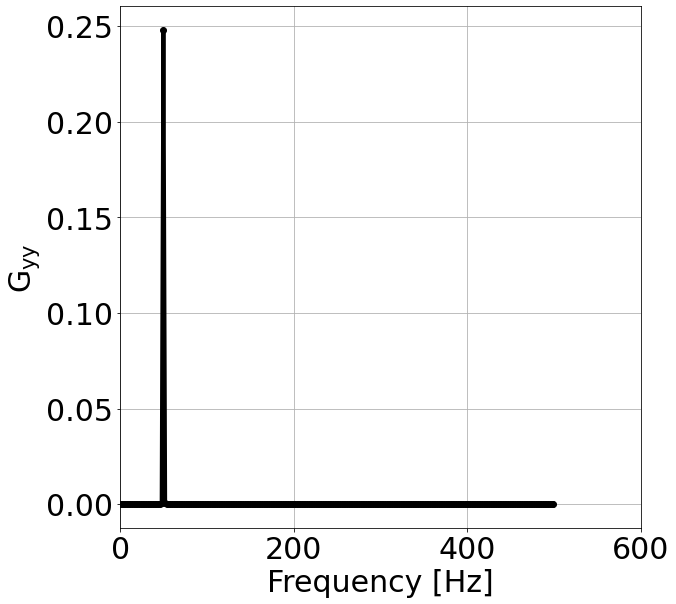
\includegraphics[width=0.5\textwidth]{./images/app_B/simple_signal_1freq_psd_single_sided_example.png}
%        \caption{Single-sided power spectrum of the signal shown in Fig.~\ref{fig:signal_and_DFT_example}(a).}
%        \label{fig:psd_example_single_sided}
%\end{figure}

\subsubsection*{Normalisation factor for the power spectral density of a discrete-time signal}\label{appendix_dft_normalisation}
This paragraph, discusses the choice of the normalisation factor $C_\mathrm{PSD}=1/(N^2 \Delta f)$ for the power spectral density of a discrete-time signal defined in Eq.~\eqref{eq:Sxx_definition_discrete_not_normalised}.

The discussion here is limited to noise signals with mean zero. This is justified since this conditions is valid for the noise spectra considered in the thesis. In particular the mean of the white noise spectra used in the simulation studies is zero by definition. The mean of the measured noise signal corresponds to the DC componenet which for the spectra discussed in this thesis was also at 0\,Hz.

Consider the example of a discrete-time series $y_n = y(n\Delta t)$ where $n$ is an integer such that $n \in [0, N-1]$. $y_n$ represents a sequence of successive points equally spaced in time, with zero mean, $\mu=0$. The variance of this collection of $N$ equally spaced values is given by:

%drawn from a normal distribution with known standard deviation $\sigma$ and zero mean, $\mu=0$. The variance of this collection of $N$ equally spaced values is given by:
\begin{equation}\label{eq:variance}
    \sigma^2 = \frac{1}{N}\sum_{n=0}^{N-1} \left | y_n \right |^2.
\end{equation}
According to Parseval's theorem~\cite{FFT_and_applications}, the variance can be written as:
%p.112
\begin{equation}\label{eq:variance_2}
    \sigma^2 = \frac{1}{N^2}\sum_{k=-\frac{N-1}{2}}^{\frac{N-1}{2}} \left | \fourierxform{y}_k \right |^2,
\end{equation}
where $\fourierxform{y}_k$ is the discrete Fourier transform of $y_n$.

Using Eq.~(\ref{eq:Sxx_definition}), the autocorrelation function $R_{yy}(\tau)$ for a continuous-time signal can be found from the inverse Fourier transform of $S_{yy}(f)$:
\begin{equation}\label{eq:autocorrelation_ivnerse}
R_{yy}(\tau) = \int_{-\infty}^{\infty} \bar{y}(t) y(t+\tau) \, dt = \int_{-\infty}^{\infty} S_{yy}(f) e^{2\pi \imagunit t f} \, df.
\end{equation}
For zero lag, this becomes:
\begin{equation}\label{eq:autocorrelation_zero_lag}
R_{yy}(0) = \int_{-\infty}^{\infty} S_{yy}(f) \, df = \sigma^2.
\end{equation}
This expresses the fact that the autocorrelation of a zero-mean stochastic process (such as $y_n$) is equal to the variance. It should be noted here that this integration over the spectral components yields the total power of the process.

For a discrete-time signal, we require that the power spectral density $S_{yy}(f_k)$ corresponds to the power spectral density for the continuous-time signal. In that case, Eq.~\eqref{eq:autocorrelation_zero_lag}
becomes:
\begin{equation}\label{eq:autocorrelation_zero_lag_discrete}
\sigma^2 =  \sum_{k=-\frac{N-1}{2}}^{\frac{N-1}{2}} S_{yy}(f_k) \Delta f.
\end{equation}

From Eq.~(\ref{eq:variance_2}) and Eq.~(\ref{eq:autocorrelation_zero_lag_discrete}) this leads to:
\begin{equation}\label{eq:normalisation_test}
 \frac{1}{N^2}\sum_{k=-\frac{N-1}{2}}^{\frac{N-1}{2}} \left | \fourierxform{y}_k \right |^2 =  \sum_{k=-\frac{N-1}{2}}^{\frac{N-1}{2}} S_{yy}(f_k) \Delta f,
\end{equation} %\Rightarrow \\
and hence:
\begin{equation}
  \sum_{k=-\frac{N-1}{2}}^{\frac{N-1}{2}} \frac{\left | \fourierxform{y}_k \right |^2}{N^2 \Delta f} =  \sum_{k=-\frac{N-1}{2}}^{\frac{N-1}{2}} S_{yy}(f_k).
\end{equation}
Therefore, to satisfy the requirement that the power spectral density for the discrete-time signal corresponds to that for the continuous-time signal, we define the power spectral density for a discrete-time signal:
\begin{equation}
    S_{yy}(f_k) = \frac{\left | \fourierxform{y}_k \right |^2}{N^2 \Delta f}.
\end{equation}
Hence, the normalisation factor in Eq.~\eqref{eq:Sxx_definition_discrete_not_normalised} is chosen to be:
\begin{equation}
    C_\mathrm{PSD}=\frac{1}{N^2 \Delta f}.
\end{equation}

\textbf{Computation of power spectral density for white noise signals}\\
At this point it is worth elaborating on the computation of the power spectral density, in the context of the noise effects in a synchrotron that are studied in this thesis.

In Chapter~\ref{Ch:CC_noise_theory} it was discussed that the noise effects are modeled as kicks which update the angle co-ordinates of the particles and which are applied to them once per turn and thus they consist of a discrete-time signal. The power spectral density of that noise signal is given by Eq.~\eqref{eq:autocorrelation_zero_lag_discrete}.  Now, given the fact that in an accelerator the particles receive the noise kicks once per turn, the sampling frequency, $f_s$ equals the revolution frequency, $\frev$. This means that the frequency resolution, $\Delta f$, can be written as $\Delta f = f_s/N = \frev/N$, where $N$ is the number of samples (or size) in the noise signal. 

Furthermore, the studies consider white noise, which is a random signal with the same amplitude (intensity) at all the frequencies which results in a uniform power spectral density. The white noise can be treated in the discrete-time domain as a sequence of uncorrelated random variables taken from a Gaussian distribution with mean zero and finite standard deviation, $\sigma_\mathrm{white}$.  Since by definition the power spectral density (for white noise signal) is the same in every frequency, Eq.~\eqref{eq:autocorrelation_zero_lag_discrete} is re-written as:
\begin{equation}\label{eq:psd_for_white_noise_variance_v0}
    \sigma_\mathrm{white}^2 =  N S_{yy}(f_k) \frev/N = S_{yy}(f_k) \frev,
\end{equation}
which becomes:
\begin{equation}\label{eq:psd_for_white_noise_variance}
   S_{yy}(f_k) = \frac{\sigma_\mathrm{white}^2 } {\frev}.
\end{equation}


In other words, the power spectral density at a given frequency, $f_k$, for a white noise spectrum modeled as described above, equals the variance of the noise signal over the revolution frequency in the synchrotron.

%\section{Measuring amplitude and phase noise}\label{app:Measured_noise}
%Amplitude and phase modulation are two of the main types of noise in the output signal of an oscillator. The instantaneous output voltage of an ideal oscillator can be expressed as:
%\begin{equation}
%    V(t) = V_0 \sin(2\pi f_0 t),
%\end{equation}
%where $V_0$ is the nominal peak voltage amplitude and $f_0$ the nominal frequency. 

%However, in practice, small inaccuracies will introduce amplitude and phase modulations. These modulations are included in the above signal by adding stochastic processes, represented by $\phi(t)$ and $\epsilon (t)$, as follows:
%\begin{equation}\label{eq:Oscillator_PN_AN}
%    \begin{split}
 %   V(t) = &~(V_0+\epsilon(t)) \sin(2\pi f_0 t + \phi(t)), \\
 %   = &~\left( 1+\frac{\epsilon(t)}{V_0} \right) V_0 \sin(2\pi f_0 t + \phi(t)), \\ =  &~(1+\alpha(t)) V_0 \sin(2\pi f_0 t + \phi(t)),
 %   \end{split}
%\end{equation}
%where $\phi(t)$ is the deviation from the nominal phase $2\pi f_0 t$, $\epsilon(t)$ is the deviation from the nominal amplitude and $\alpha(t)=\epsilon(t)/V_0$ is the normalised amplitude deviation.  An example of a signal with phase and amplitude noise is shown in Fig.~\ref{fig:AN_PN_example}. 

%\begin{figure}[!ht]
%    \centering
%    \begin{subfigure}[b]{0.45\textwidth}
%        \centering
%        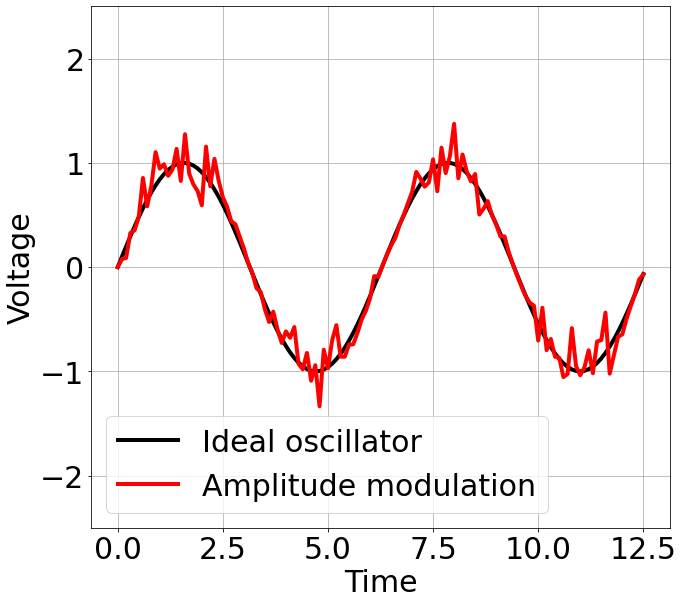
\includegraphics[width=1\textwidth]{./images/app_B/oscillator_example_AN.png}
%        \caption{Amplitude noise}
%        \label{fig:AN_PN_example_a}
 %   \end{subfigure}
 %   \hfill
 %   \begin{subfigure}[b]{0.45 \textwidth}
 %       \centering
 %       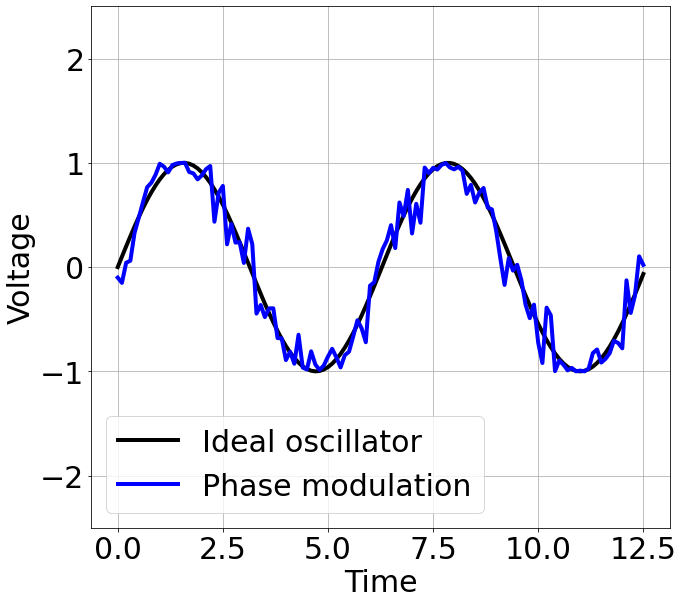
\includegraphics[width=1 \textwidth]{./images/app_B/oscillator_example_PN.png}
 %       \caption{Phase noise}
 %       \label{fig:AN_PN_example_b}
 %   \end{subfigure}
 %   \hfill
 %   \begin{subfigure}[b]{0.45\textwidth}
 %       \centering
 %       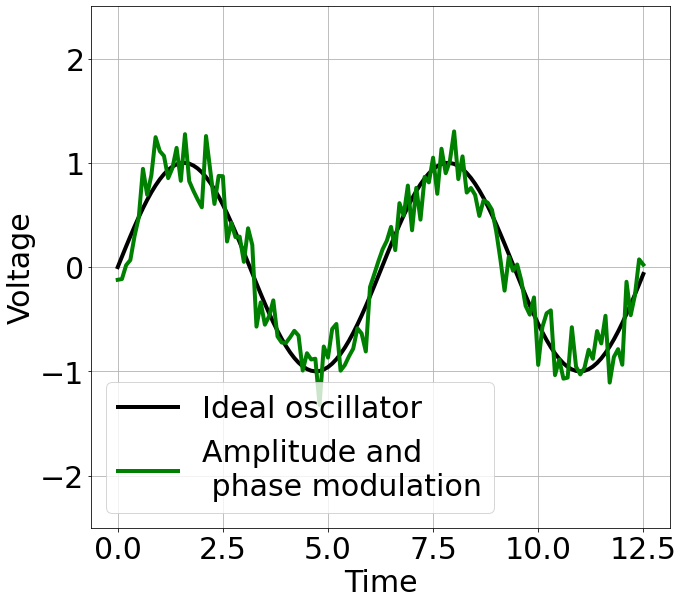
\includegraphics[width=1\textwidth]{./images/app_B/oscillator_example_AN_PN.png}
 %       \caption{Amplitude and phase noise}
 %       \label{fig:AN_PN_example_c}
 %   \end{subfigure}
 %   \hfill
 %   \caption{Instantaneous voltage of an oscillator in the presence of (a) amplitude noise, (b) phase noise, and (c) both amplitude and phase noise.}
%    \label{fig:AN_PN_example}
%\end{figure}

%Following the IEEE~\cite{IEEE:4797525} conventions, the amplitude and phase modulation are measured by one-sided spectral densities, $G_{yy}(f)$. From Eq.~(\ref{eq:Sxx_definition_discrete_normalized}) and Eq.~(\ref{eq:two-sided_2_single-sided}), the amount of amplitude noise can be expressed as:
%\begin{equation}\label{eq:AN_measure}
%    G_\alpha(f_k) = 2 S_a(f_k)=\frac{2}{N^2 \Delta f} \left (  \frac{\mid\fourierxform{\epsilon}(f_k)\mid}{V_0} \right ) ^2=\frac{2}{N^2\Delta f } \mid \fourierxform{\alpha}(f_k) \mid ^2,
%\end{equation}
%and the amount of phase noise can be expressed:
%\begin{equation}\label{eq:PN_measure}
%    G_\phi(f_k) = 2 S_\phi(f_k)=\frac{2}{N^2 \Delta f} \mid \fourierxform{\phi}(f_k) \mid ^2,
%\end{equation}
%where $f_k$ lies in a range of positive frequencies and $\fourierxform{\alpha}(f_k)$ and $\fourierxform{\phi}(f_k)$ are the discrete Fourier transforms of the modulation signals $\alpha(t)$ and $\phi(t)$ respectively. The units of the $G_\alpha(f_k)$ are 1/Hz and the units of $G_\phi(f_k)$ are rad$^2$/Hz.
% Initially $G_\alpha(f_k)$ are $V^2$/Hz but changed to 1/Hz (which is also in accordance with the paper of themis and philippe, as it is relative to the V--> unitless) on 29 July 2022.

%However, instruments used in experiments do not usually display directly the single-sided spectral density $G_{yy}$. Instead, the quantity $10\log_{10}\mathcal{L}(f_k)$\,[dBc/Hz] is shown, with~\cite{IEEE:4797525}:
%\begin{equation}\label{eq:L_to_G}
%    \mathcal{L}(f_k) = G_{yy}(f_k)/2,
%\end{equation}
%where $f_k$ ranges from 0 over the positive part of the spectrum. It should be emphasised that here $\mathcal{L}$ is two-sided, as defined in~\cite{IEEE:4797525}, though it is considered that the instrument displays only the positive frequencies.

%\section{Applying a measured noise spectrum in numerical simulations}\label{sec:measured_spectra_to_time_series}

%This section discusses the steps required to convert a measured noise spectra to a discrete-time series i.e. a sequence of noise kicks, that can be used in tracking simulations. 

%The goal of this section is to describe how one can convert the measured noise spectrum from a spectrum analyzer to a discrete time series that can be used in numerical simulations. % Recall, that the phase and amplitude noise are modeled in the tracking simulations as sequences of noise kicks which change the transverse angle co-ordinate of the particles each turn (see  Eqs.~\eqref{eq:amplitude_noise_kick},~\eqref{eq:phase_noise_kick} and~\eqref{eq:CC_kick_sixtracklib_vertical_noise}).



%\subsection{Crab cavity noise in numerical simulations}
%As discussed in Chapter~\ref{Ch:CC_noise_theory} the phase and amplitude noise are modeled in the tracking simulatiosn as sequences of noise kicks which change the transverse angle co-ordinate of the particles each turn. These discrete time series can be representated by $\alpha_n = \alpha(n\Delta t)$ and  $\phi_n = \phi(n\Delta t)$ for amplitude and phase noise, respectively, where  $n \in \left [1, N_\mathrm{turns}-1 \right ]$ and $N_\mathrm{turns}$ is the number of turns in the simulation.



%Since in the simulations the beam encounters the phase or amplitude noise kicks once per turn, the sampling frequency of the noise spectra $f_s$ equals the revolution frequency (see discussion in Chapter~\ref{Ch:investigating_discrepancy}). For, the SPS $f_s=\frev=43/73$ \,kHz. Hence, the sampling interval should be $\Delta t=1/f_s = 1/\frev \approx$ 23 $\mathrm{\mu s}$.  


%, representated by 
%$\alpha_n = \alpha(n\Delta t)$ and  $\phi_n = \phi(n\Delta t)$ for amplitude and phase noise respectively, that can be applied in the numerical simulations, following Eqs.~\eqref{eq:amplitude_noise_kick},~\eqref{eq:phase_noise_kick} and~\eqref{eq:CC_kick_sixtracklib_vertical_noise}. To apply the mesaured noise spectra in the simulations, the parameters $\Delta A_j$ and $\Delta \phi_j$ introduced in the above equations will correspond to the $j^\mathrm{th}$ element of the $\alpha_n$ and $\phi_n$, respectively.

%The goal of this section is to describe how one can convert the measured noise spectrum from a spectrum analyzer to a discrete time series, representated by 
%$\alpha_n = \alpha(n\Delta t)$ and  $\phi_n = \phi(n\Delta t)$ for amplitude and phase noise respectively, that can be applied in the numerical simulations, following Eqs.~\eqref{eq:amplitude_noise_kick},~\eqref{eq:phase_noise_kick} and~\eqref{eq:CC_kick_sixtracklib_vertical_noise}. To apply the mesaured noise spectra in the simulations, the parameters $\Delta A_j$ and $\Delta \phi_j$ introduced in the above equations will correspond to the $j^\mathrm{th}$ element of the $\alpha_n$ and $\phi_n$, respectively.


%For the correct implementation in numerical simulations, $n \in \left [1, N_\mathrm{turns}-1 \right ]$ and $N_\mathrm{turns}$ is the number of simulated turns. Furthermore, in the simulations the beam enounters the phase or amplitude noise kicks once per turn. This means that the sampling frequency, $f_s=\frev$ which for the SPS is 43.47\,kHz. Hence, the sampling interval should be $\Delta t=1/f_s = 1/\frev \approx$ 23 $\mathrm{\mu s}$. 


%The dicrete time series for amplitude and phase noise are representated by $\alpha_n = \alpha(n\Delta t)$ and  $\phi_n = \phi(n\Delta t)$ respectively.

%, as shown in Eqs.~\eqref{eq:amplitude_noise_kick},~\eqref{eq:phase_noise_kick} and~\eqref{eq:CC_kick_sixtracklib_vertical_noise}. This time, $\Delta A_j$ and/or $\Delta \phi_j$ were not drawn from a Gaussian distribution of size equal the number of simulation turns, $N_\mathrm{turns}$, with zero mean and a given standard deviation as for the case of white noise.


%%%%%%%%%%



%\subsection{Crab cavity noise in numerical simulations}
%As follows from the discussion in section~\ref{subsec:Measured_noise}, phase and amplitude noise can be represented by discrete time series $\phi_n = \phi(n\Delta t)$ and  $\alpha_n = \alpha(n\Delta t)$ respectively, so that the crab cavity (CC) instantaneous voltage is given by:
%\begin{equation}\label{eq:CC_PN_AN}
%    \VCC (n \Delta t) =  V_0(1+\alpha(n \Delta t)) \sin{(2\pi f_0 n \Delta t + \phi(n \Delta t)},
%\end{equation}
%where $V_0$ and $f_0$ are the nominal crab cavity voltage and frequency respectively, $n \in \left [1, N-1 \right ]$ and $N$ is the number of samples.

%In numerical simulations, $N$ is taken to be equal to the number of turns in the simulation. The total time simulated is $T=N \Delta t$, where $\Delta t$ is the sampling interval. Since the phase and amplitude noise are sequences of noise kicks which are applied to the CC voltage every turn, $\Delta t$ is equal to the time needed for one turn around the machine. For the SPS, with a revolution frequency $\frev = $43.38 kHz, $\Delta t=1/f_s = 1/\frev \approx$ 23 $\mathrm{\mu s}$. 
%%%%%%%%%%%

%\subsection{Measured noise spectrum}

%As discussed in Section~\ref{sec:injected_RF_noise}, the noise spectra discussed in this thesis, were measured with a spectrum analyzer E5052B~\cite{E5052B_insight} and are expressed as $10\log_{10}\mathcal{L}(f)$\,[dBc/Hz], where $\mathcal{L}(f)$ follows the IEEE definitions in~\cite{IEEE:4797525}. Recall that $\mathcal{L}(f)$ as defined in~\cite{IEEE:4797525} is two-sided, which means that it has both positive and negative frequencies and as a real signal is symmetric around the DC component, $f=0$\,Hz. However, since the spectrum analyser E5052B displays the logarithmic quantity $10\log_{10}\mathcal{L}(f)$ only the positive frequencies are displayed (see Fig.~\ref{fig:coast1_setting2_a}).

%The relation between the measured noise levels and the power spectral densities in Eq.~\eqref{eq:dey_an} and Eq.~\eqref{eq:dey_pn} following the IEEE conventions~\cite{IEEE:4797525} is given by $S_{\Delta A, \Delta \phi}(f) = \mathcal{L}(f)$ (see Table A.1 in~\cite{IEEE:4797525}), with $S_{\Delta A}$ in\,Hz$^{-1}$ and $S_{\Delta \phi}$ in $\mathrm{rad^2 Hz^{-1}}$. 


%\subsection{Generating time series}\label{subsec:generatin_noise_kicks}
%In the following, the steps required to generate the discrete time series $\alpha_n$ and $\phi_n$ from the measured noise spectrum are discussed. The procedure involves converting the measured noise power to the two-sided power spectral density $S_\phi(f_k)$ and then using the inverse Fourier transform to produce the discrete-time series of noise kicks. In detail, the steps are as follows:

\section{Applying a measured noise spectrum in numerical simulations}\label{sec:measured_spectra_to_time_series}

This section discusses the steps required to convert a measured noise spectra to a discrete-time series i.e. a sequence of noise kicks, that can be used in tracking simulations. For the discussion an example phase noise spectra measured during the $\CC$ tests in SPS in 2018 are discussed (see Fig.~\ref{fig:coast1_setting2_a}). Note that the steps are the same for an amplitude noise spectra. The procedure involves converting the measured noise power to the power spectral density and then using the inverse Fourier transform to produce the discrete-time series of noise kicks. 

In detail, the steps are as follows:

\begin{enumerate}
    \item  Convert the measured noise power $10\log_{10}\mathcal{L}(f_k)$\,[dBc/Hz] to the power spectral density, $S_{\Delta \phi}(f_k)$, recalling that $S_{\Delta \phi}(f_k) = \mathcal{L}(f_k)$ (see Section~\ref{sec:injected_RF_noise}). This is shown in Fig.~\ref{fig:coast1_setting2_b}. For now the analysis is limited to $f_k \in [1, 10^{3}]$\,kHz. Note, that both $\mathcal{L}(f_k)$ and $S_{\Delta \phi}(f_k)$ have both negative and positive components and are symmetric around the DC component, $f_k=0$\,Hz (see Section~\ref{sec:injected_RF_noise}).

    %$G_\phi(f_k)$\,[$\mathrm{rad^2}$/Hz] using Eq.~(\ref{eq:L_to_G}) (Fig.~\ref{fig:coast1_setting2_b}).
    \item Re-sample the noise spectrum. The measured noise power values are equally spaced in frequency on a logarithmic scale. A linear interpolation is needed such that they are equally spaced on a linear scale, every $\Delta f = f_s/N$. As discussed in Section~\ref{sec:benchmark_theory_with_pyheadtail} since the beam encounters the noise once per turn, the sampling frequency of the noise spectrum in the simulations equals the revolution frequency, $f_s=f_\mathrm{rev}(=43.38$ kHz for the SPS). Note that the frequency spectrum of the noise in the simulations and hence the linear interpolation extends up to $f_s/2$ as illustrated in Fig.~\ref{fig:coast1_setting2_c}. In our simulations, $N=10^5$ turns are used. The result is shown in Fig.~\ref{fig:coast1_setting2_c}.
    %\item Create the positive spectral components of the two-sided power spectrum, $S_\phi$, using Eq.~(\ref{eq:two-sided_2_single-sided}) for $f_k>0$. The result is shown in Fig.~\ref{fig:coast1_setting2_d}.
    \item Compute the amplitude of the spectral components of the Fourier transform, $\left | \fourierxform{\phi}_n(f_k) \right | $ according to Eq.~(\ref{eq:Sxx_definition_discrete_normalized}). %It should be noted, however, that this computation is done only for the positive part of the spectrum. Fig.~\ref{fig:coast1_setting2_e} depicts the result of this computation. 
    \item Generate the phase information for each positive spectral component. By definition the power spectral density does not contain any information about the phase of the frequency components. Therefore, one should generate this information by giving a random phase $\theta(f_k)$ obtained from uniform distribution between 0 and $2\pi$.
    \item Construct a one-sided frequency domain signal, $\fourierxform{\phi}_n^\mathrm{os}(f_k) =\left| \fourierxform{\phi}_n(f_k) \right| e^{\imagunit \theta(f_k)}$.  Once again this computation is done only for the positive spectral components, with $f_k \in \left[\Delta f,+\frac{f_s}{2} \right ]$.
    \item Construct the two-sided Fourier transform spectrum. First, create the negative components of the Fourier transform by taking the complex conjugate of the positive components. Furthermore, the information for the zero frequency component (DC) is missing from the measured spectrum, since this extends from  1 kHz to 10 MHz. In order to do the conversion correctly, the zero frequency term is set to 0, so that $\fourierxform{y}_n(0)=0$. The two-sided Fourier transform is then given by:
    

    \begin{equation}
        \fourierxform{\phi}_n(f_k) = = \left\{\begin{matrix}
   \left | \fourierxform{\phi}_n^\mathrm{os}(f_k) \right | \overline{e^{\imagunit\theta (\mid f_k \mid)}}, & f_k \in \left [-\frac{f_s}{2}, -\Delta f_s \right] \\ 
    \left | \fourierxform{\phi}_n^\mathrm{os}(f_k) \right | = 0, & f_k=0  \\
   \left | \fourierxform{\phi}_n^\mathrm{os}(f_k) \right | e^{\imagunit\theta (\mid f_k \mid)}, & f_k \in \left [+ \Delta f_s, + \frac{f_s}{2} \right]  
    \end{matrix}\right.
    \end{equation}

    It is clear that $\fourierxform{\phi}_n(f_k)$ has both positive and negative frequencies and the magnitude is symmetric in $f_k$.
    
    \item Finally, apply the inverse Fourier transform, Eq.~(\ref{eq:iDFT_definiton}), to $\fourierxform{\phi}_n(f_k)$. The  output  is  a  random  discrete  time  series of $N$ values sampled every $\Delta t = 1/f_s=1/f_{rev}$. In other words, $\phi_n$ forms the sequence of noise kicks that will act on the particles in the beam on each turn in the simulations.

\end{enumerate} 

%Path to plotting script: cernbox/Project_thesis/scripts_for_simple_figures_plot/measured_psd_to_time_series
\begin{figure}[!ht]
    \centering
    \begin{subfigure}[t]{0.42\textwidth}
        \centering
        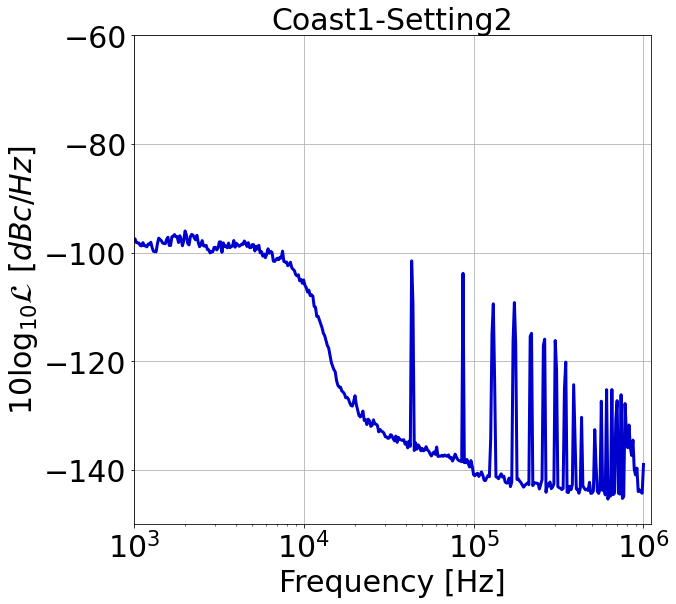
\includegraphics[width=1\textwidth]{./images/app_B/coast1_setting2_v1.png}
        \caption{Phase noise spectrum measured with a spectrum analyzer E5052B.}
        \label{fig:coast1_setting2_a}
    \end{subfigure}
    \hfill
    \begin{subfigure}[t]{0.42\textwidth}
        \centering
        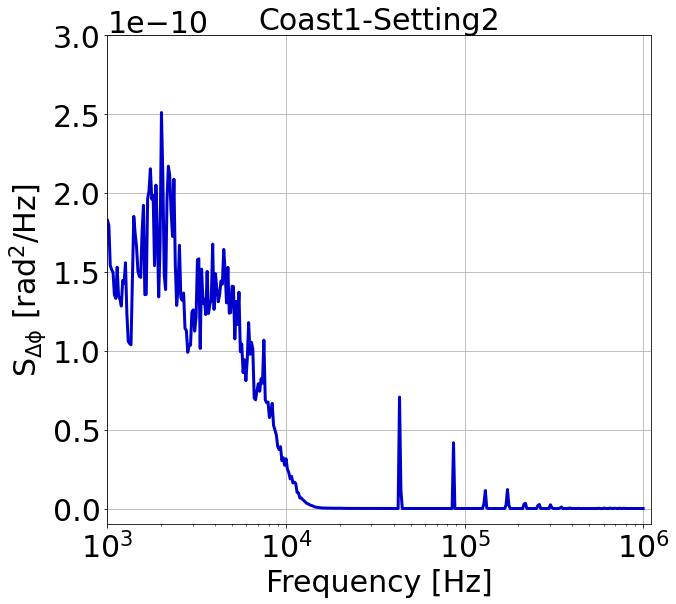
\includegraphics[width=1 \textwidth]{./images/app_B/coast1_setting2_v2.png}
        \caption{Measured phase noise spectrum in  units rad$^2$/Hz.}
        \label{fig:coast1_setting2_b}
    \end{subfigure}
    \hfill
    \begin{subfigure}[t]{0.42\textwidth}
        \centering
        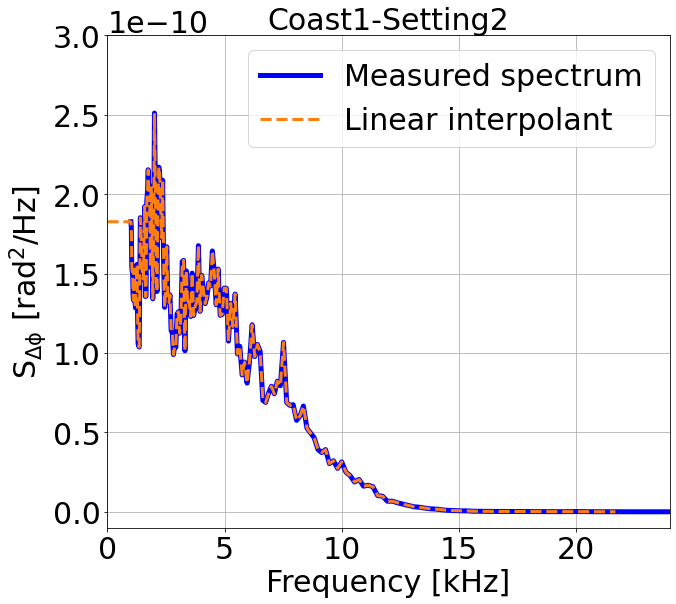
\includegraphics[width=1\textwidth]{./images/app_B/coast1_setting2_v3.png}
        \caption{Linear interpolation of the measured noise spectrum. %sampled every $\Delta f = f_{rev}/N$. Here $f_{rev}$=43.45 [kHz] and N=$10^5$ turns are used.}
        }
        \label{fig:coast1_setting2_c}
    \end{subfigure}
    \hfill
    \begin{subfigure}[t]{0.42\textwidth}
        \centering
        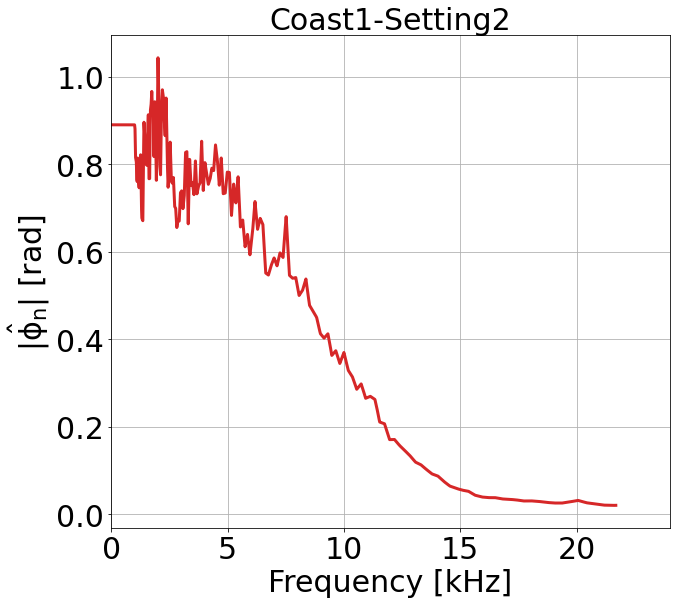
\includegraphics[width=1\textwidth]{./images/app_B/coast1_setting3_v4.png}
        \caption{Amplitudes of the spectral components of the Fourier transform.}
        \label{fig:coast1_setting2_d}
    \end{subfigure}
    \hfill
    \centering
    \begin{subfigure}[t]{0.42\textwidth}
        %\hspace{3.5cm} % manually move the figure to the center. But caption doesn't move
        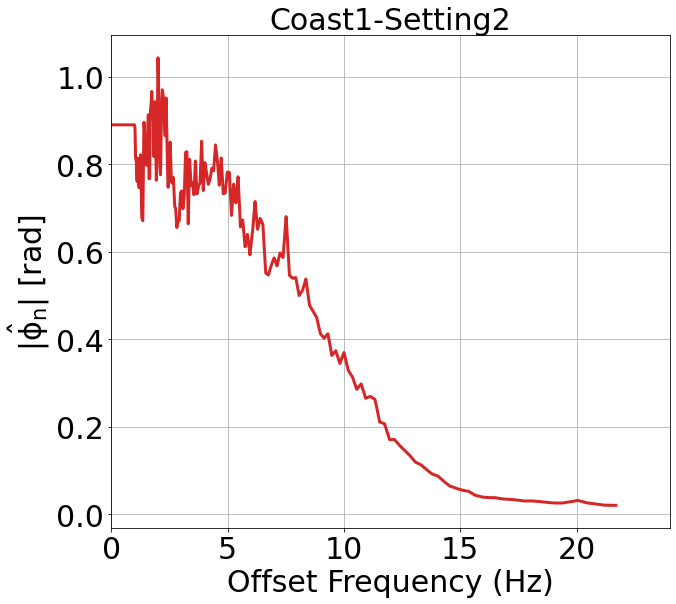
\includegraphics[width=1\textwidth]{./images/app_B/coast1_setting2_yn_fft.png}
        \caption{Amplitudes of the spectral components of the Fourier transform. %sampled every $\Delta f = f_{rev}/N$. Here $f_{rev}$=43.45 [kHz] and N=$10^5$ turns are used.}
        }
        \label{fig:coast1_setting2_e}
    \end{subfigure}
    \hfill
    %\begin{subfigure}[b]{0.45\textwidth}
    %    \centering
    %    \includegraphics[width=1\textwidth]{coast1_setting2_generated_phase_noise_kicks.png}
    %    \caption{Sequence of phase noise kicks generated from the measured power spectrum of Fig.~\ref{fig:coast1_setting2_a}}
    %    \label{fig:coast1_setting2_f}
    %\end{subfigure}
    %\hfill
    \hfill
    \caption{Steps required to generate the sequence of noise kicks to be applied in the simulations from the measured noise spectrum.}
    \label{fig:noise_kick_generation}
\end{figure}


\subsection{Validation of the time series reconstruction}
This section describes the benchmarks that were carried out to ensure that the method described in section \ref{subsec:generatin_noise_kicks} produces a valid time series for a set of noise kicks, for a given power spectrum. 

\subsubsection*{Comparison of measured and reconstructed power spectrum} %\hfill \break
Figure \ref{fig:generate_noise_kicks_sanity_check_1} shows the results of the first benchmark, comparing the measured power spectral density with the power spectral density computed from the generated time series $\phi_n$. The two power spectra appear to be consistent with each other, which supports the validity of the method described above for generating the sequence of noise kicks from a given power spectrum. 

\begin{figure}[!ht]
     \centering         
     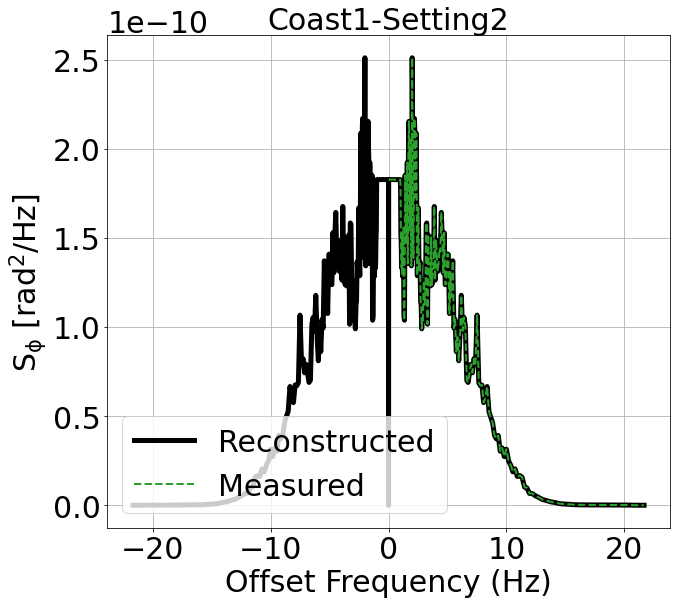
\includegraphics[width=0.5\textwidth]{./images/app_B/coast1_setting2_Syy_original_vs_reconstructed_sanity_check.png}
         \caption{Power spectral density computed from the time series $\phi_n$ produced from a measured power spectrum (black), compared with the original measured power spectrum (green).}
         \label{fig:generate_noise_kicks_sanity_check_1}
\end{figure} 

\subsubsection*{PyHEADTAIL simulations} %\hfill \break
Another way to validate the method for producing a sequence of noise kicks from a measured power spectrum is to perform numerical simulations using the generated noise kicks, and compare the resulting emittance growth with the predictions form an analytical model~\cite{PhysRevSTAB.18.101001}.

In the simulations, which were performed with PyHEADTAIL, the beam was tracked for $10^5$ turns which corresponds to about 2.5\,s in the SPS. A kick representing the effect of the crab cavities was applied on each turn. The noise kicks that the beam encounters every turn at the CC location were generated from the phase and amplitude noise spectra of from Coast1-Setting2 of 2018 (Fig.~\ref{fig:example_PN_and_AN_coast1_setting2}). 

It should be noted, however, that the sequence of noise kicks includes a random factor through the set of random phases $\theta(f_k)$. To reduce the uncertainty in the results, multiple simulation runs were conducted. The set of random phases was regenerated randomly for each of 10 runs with a different seed each time. For each run, the initial bunch distribution was also regenerated randomly 3 times. The mean and the standard deviation of the emittance values obtained from the tracking were computed over all trials. The emittance growth rate was computed by performing a linear fit to the mean of the emittance values.

Figures~\ref{fig:emitGrowth_AN} and~\ref{fig:emitGrowth_PN} show the emittance growth for the case of amplitude noise and phase noise respectively. The emittance evolution in the presence of both types of noise is also illustrated in Fig.~\ref{fig:emitGrowth_AN_and_PN}. The simulated emittance growth rates show very good agreement with the predictions from the analytical model. The results again support the validity of the method for generating a sequence of noise kicks from a measured noise power spectrum, described in section \ref{subsec:generatin_noise_kicks}.


\begin{figure}[!ht]
     \centering
     \begin{subfigure}[t]{0.45\textwidth}
         \centering
         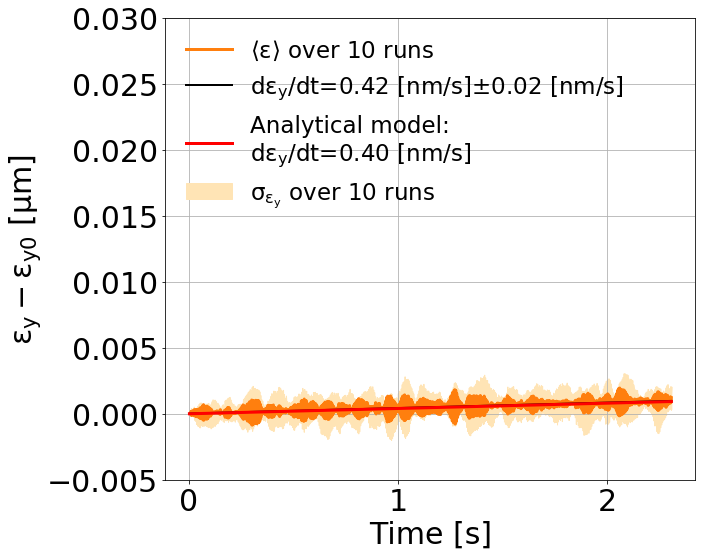
\includegraphics[width=1\textwidth]{./images/app_B/emitGrowth_eyEvolution_sps_270GeV_WakesOFF_ayy1500_QpxQpy1_Nb5e5_IPACvalues_coast1_setting2_AN.png}
         \caption{Emittance growth in the presence of amplitude noise.}
         \label{fig:emitGrowth_AN}
     \end{subfigure}
     \hfill
     \begin{subfigure}[t]{0.45 \textwidth}
         \centering
         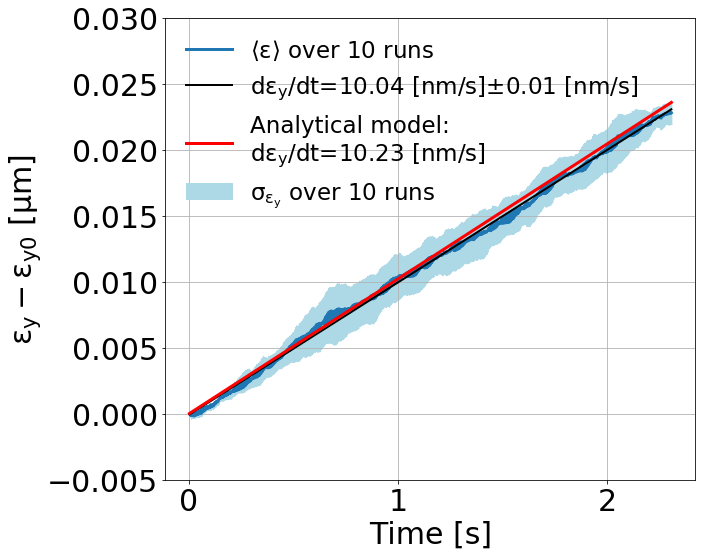
\includegraphics[width=1 \textwidth]{./images/app_B/emitGrowth_eyEvolution_sps_270GeV_WakesOFF_ayy1500_QpxQpy1_Nb5e5_IPACvalues_coast1_setting2_PN.png}
         \caption{Emittance growth in the presence of phase noise.}
         \label{fig:emitGrowth_PN}
     \end{subfigure}
     \hfill
     \begin{subfigure}[t]{0.45\textwidth}
         \centering
         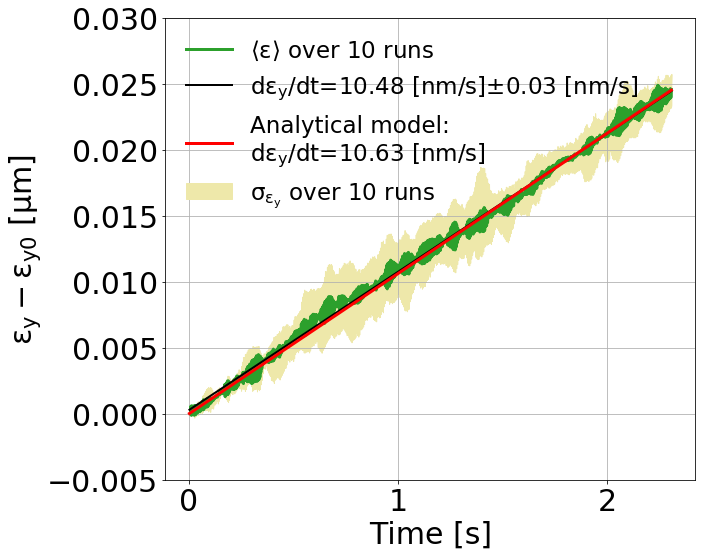
\includegraphics[width=1\textwidth]{./images/app_B/emitGrowth_eyEvolution_sps_270GeV_WakesOFF_ayy1500_QpxQpy1_Nb5e5_IPACvalues_coast1_setting2_AN_PN.png}
        \caption{Emittance growth in the presence of both amplitude and phase noise.}
         \label{fig:emitGrowth_AN_and_PN}
     \end{subfigure}
     \hfill
     \caption{Comparison between emittance growth found from simulations in PyHEADTAIL and emittance growth expected from an analytical model~\cite{PhysRevSTAB.18.101001}.  The emittance growth is driven by amplitude and phase noise, with kicks in the simulations generated from a measured power spectrum.}
     \label{fig:emitGrowth_AN_PN_example}
\end{figure}
